\chapter{Simulating Neutron Reflectivity}

This tutorial will show you how to use the ORNL LRAC Neutron Reflectivity
Simulator. Questions should be directed to billingsjj@ornl.gov.

\section{Installing the Simulator}

You may download the software from the Spallation Neutron Source (SNS) website.
Locate the file in your downloads directory. It will be named
\begin{itemize}
  \item - lrac\_reflectivity-win32.x86.zip on 32-bit Windows
  \item - lrac\_reflectivity-win32.x86\_64.zip on 64-bit Windows
  \item - lrac\_reflectivity-linux.x86.zip on 32-bit Linux
  \item - lrac\_reflectivity-linux.x86\_64.zip on 64-bit Linux
  \item - lrac\_reflectivity.mac.zip on Mac OS/X
\end{itemize}

Unzip this file to a directory of your choosing. 

\section{Getting Started}
\label{gettingStarted}

The LRAC Reflectivity Simulator works by using your data from LRAC and a
materials configuration that you provide to produce simulated
neutron reflectivity, scattering density and $RQ^4$ plots. Make sure that you
have an unaltered data file from LRAC available.

Double click the executable named lrac\_reflectivity or lrac\_reflectivity.exe
in the directory where you unzipped the download. You will be asked to provide
the name of a directory where data may be stored, (fig. \ref{workspace}.). Use the
``Browse'' button to select your preferred directory if it is not in the dropdown list. If
this is your first time using the simulator, create a new directory with no
other contents in it using the ``Browse'' button.

\begin{figure}[!h]
\centering
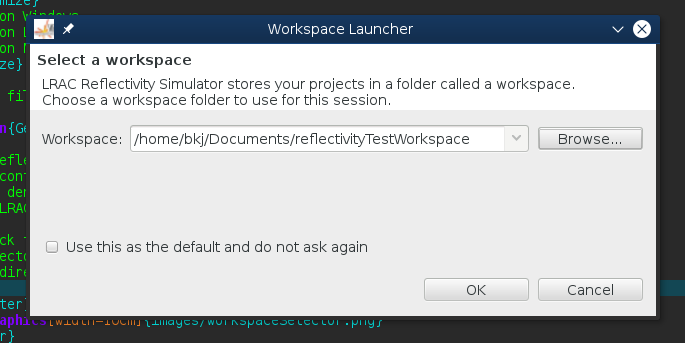
\includegraphics[width=10cm]{images/workspaceSelector.png}
\caption{The workspace selector.}
\label{workspace}
\end{figure}

Once you choose a workspace, click ``OK'' to load the simulator. You will be
presented with an empty workbench, (fig. \ref{workbench}).

\begin{figure}[!h]
\centering
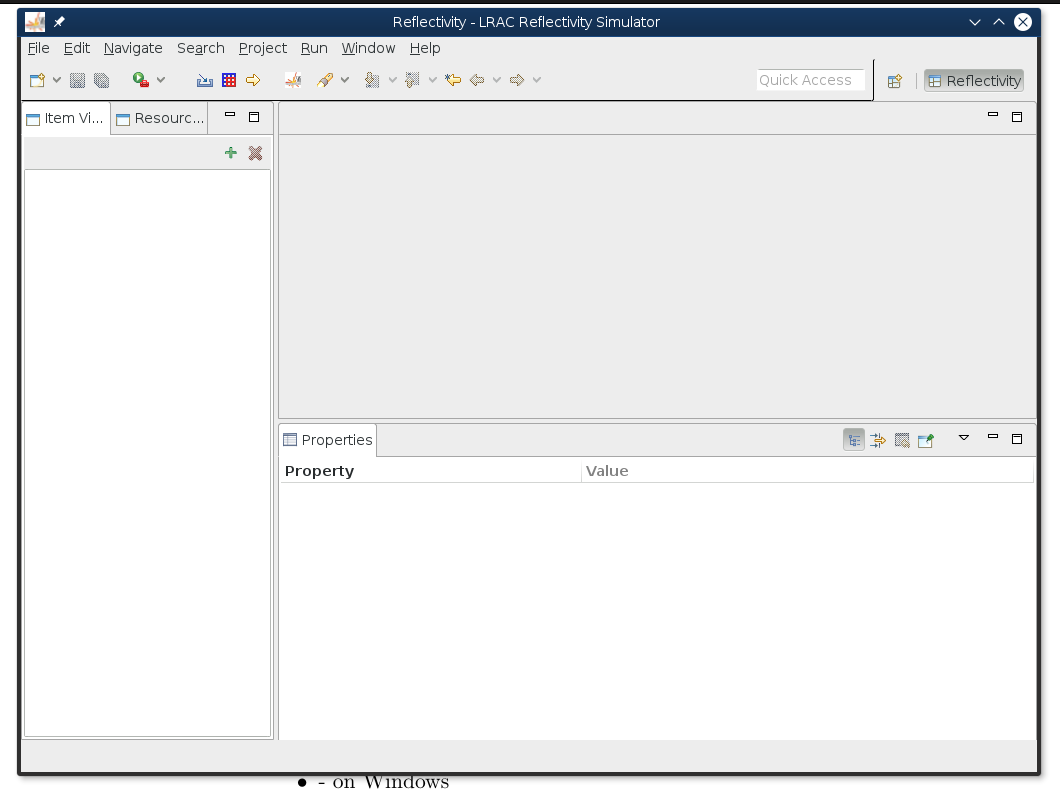
\includegraphics[width=10cm]{images/workbench.png}
\caption{The initial empty workbench.}
\label{workbench}
\end{figure}

You may run a simulation or modify materials information using the quick launch
button in the tool bar. The button is a very tiny SNS logo. Clicking it
will open a window with buttons for calculating reflectivity and modifying
materials properties, (fig. \ref{launcher}).

\begin{figure}[!h]
\centering
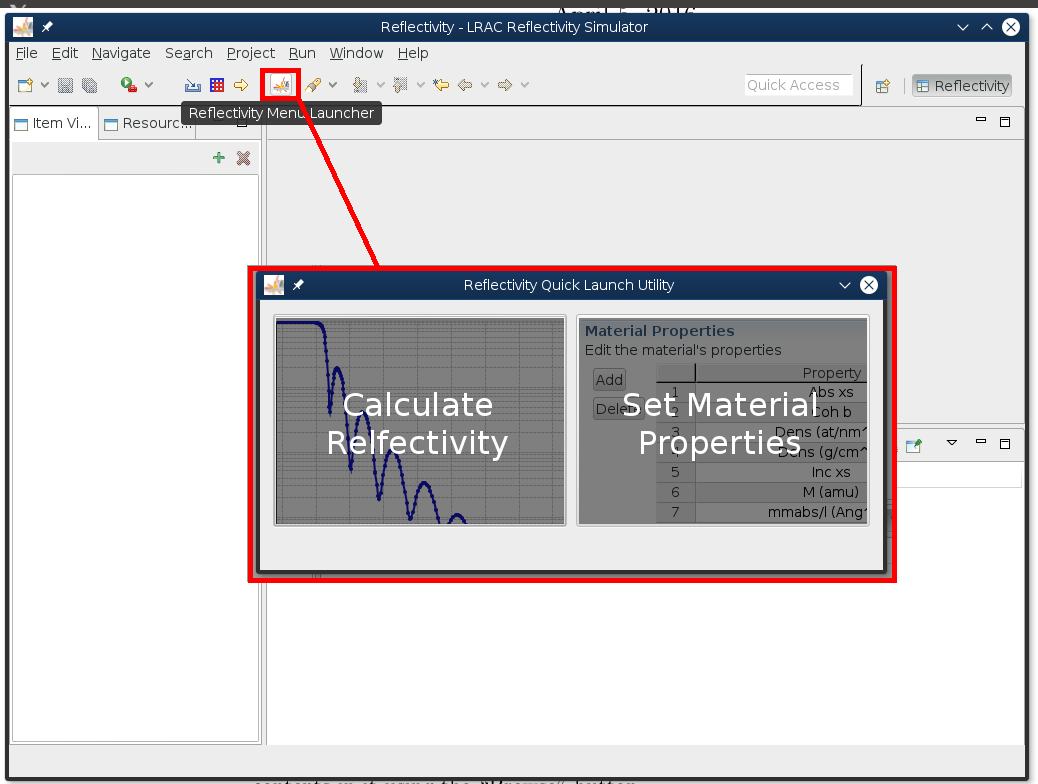
\includegraphics[width=10cm]{images/menuLauncher.png}
\caption{The Reflectivity Quick Launch menu that appears after clicking the
small SNS logo in the task bar.}
\label{launcher}
\end{figure}

Simulating reflectivity (section \ref{simulate}) and manipulating material
definitions (section \ref{modifyMaterials}) are the primary functions of the
workbench. However, the workbench is also capable of showing your data in
standalone visualizations (section \ref{viz}), and you can export your data for
your own use (section \ref{export}).

\section{Loading LRAC Data \& Simulating Reflectivity}
\label{simulate}

To load your data from LRAC and simulate the reflectivity of your material, open
the Reflectivity menu by clicking on the SNS logo in the task bar. Click the
left button labeled ``Calculate Reflectivity,'' (see fig. \ref{launcher}).
This will create a new Reflectivity Simulator for you, (fig. \ref{simulator}).

\begin{figure}[!h]
\centering
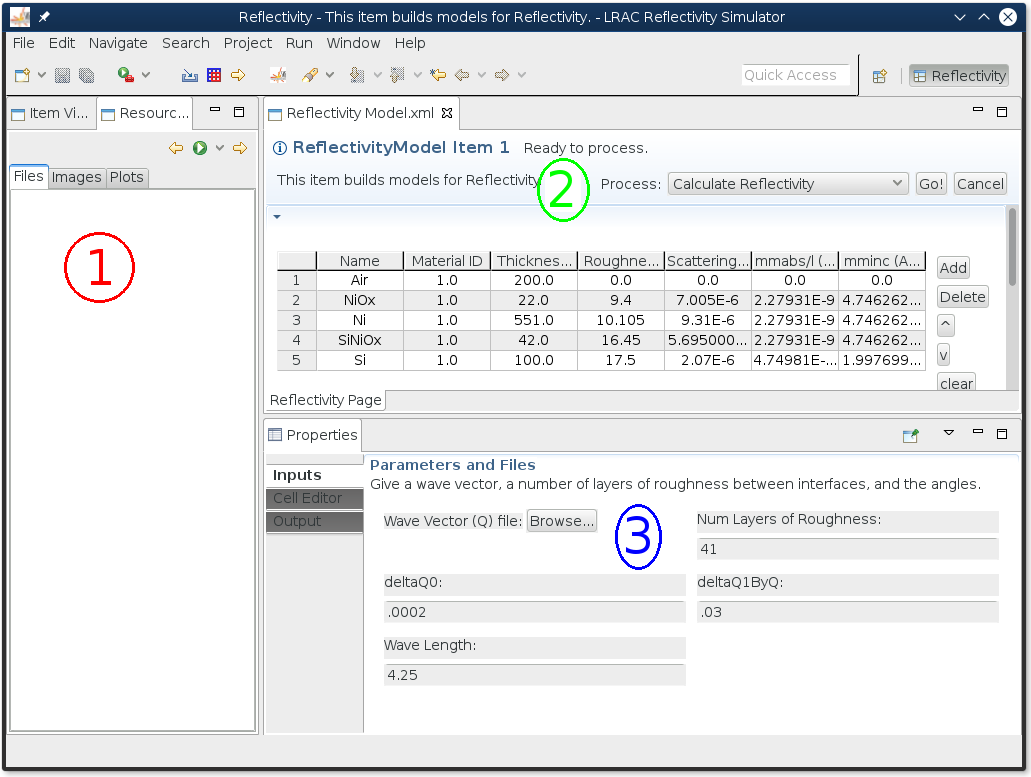
\includegraphics[width=10cm]{images/simulator_sections.png}
\caption{The reflectivity simulator with the resource view (1) on the left, the
materials table (2) on the top, and the properties view (3) on the bottom.}
\label{simulator}
\end{figure}

This workbench should now be divided into three parts. The leftmost part will be
an empty ``Resources'' menu for displaying files, images and plots. The top
right area will show a table with some layered materials listed by default. The
bottom right area will show a view labelled properties with parameters such as
``deltaQ0'' and ``Num Layers of Roughness''. (Fig. \ref{simulator} has labelled
these parts.) Each of these areas can be moved to suit your personal needs by
clicking and dragging on the tabs labelled ``Resources,'' ``Reflectivity
Model.xml,'' and ``Properties.''

In the materials table (2), a default configuration of materials is shown. You
may start to add your materials by clicking the ``Clear'' button on the right,
which will clear the table of its contents. For each layer of your sample, click
the ``Add'' button on the right. This will bring up a table of materials from
which you may choose a material that represents your layer. If your material is
not in the list, you may add that material to the database, (see section
\ref{modifyMaterials}). Continue to add layers until you have fully defined your
material. Once you are done modifying materials, click the blue ``Save'' button
in the upper left corner or hit the ``Ctrl+S'' hot key combination.

You are required to provide a data file to the Simulator that contains your wave
vector and other information provided by LRAC, including your measured
reflectivity. You may provide this data by pressing the ``Browse'' button beside
the ``Wave Vector (Q) file'' entry in the Properties View. (This is right beside
the label ``3'' in fig. \ref{simulator}.) While you are modifying properties,
make sure to change all of the properties (deltaQ0, wavelength, Num Layers of
Roughness and deltaQ1ByQ) to match your system.

You may now generate your simulated neutron reflectivity by hitting the ``Go!''
button to the upper right of the materials table. If successful, the message
``Done!'' will appear to the upper left of the materials table, three new files
should appear in the Resources menu and a ``Console'' view should appear next to
the Properties View. If you no longer need to update your properties, you may
safely minimize this view. Double clicking on one of the new entries -
Reflectivity Data File, Scattering Density Data File, or RQ$^4$ Data File - in
the Resources view will open a plot of the data beneath the materials table, (fig.
\ref{simulatorPost}).

\begin{figure}[!h]
\centering
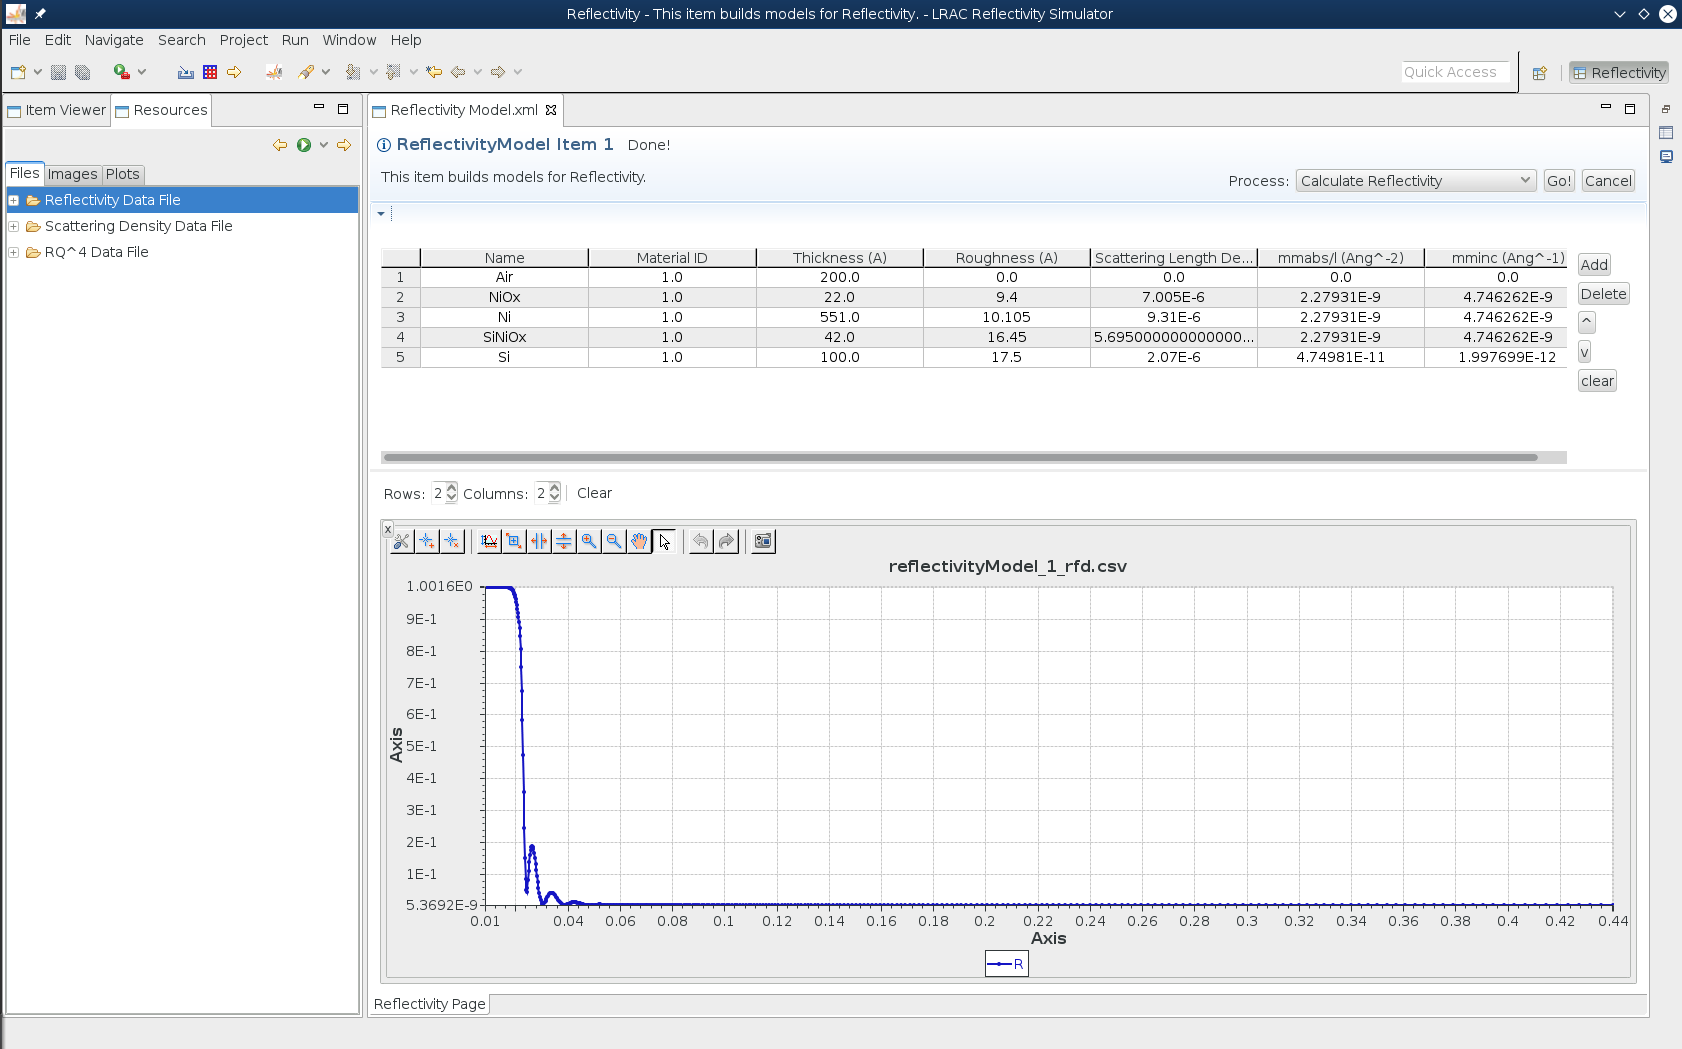
\includegraphics[width=10cm]{images/simulatorProcessed.png}
\caption{The reflectivity simulator with the resource view (1) on the left, the
materials table (2) on the top, and the properties view (3) on the bottom.}
\label{simulatorPost}
\end{figure}

\section{Adding or Removing Materials}
\label{modifyMaterials}

Custom materials can be defined by modifying the Materials Database. To add,
remove, or modify materials, open the Reflectivity menu by clicking on the SNS
logo in the task bar. Click the right button labeled ``Set Material
Properties,'' (see fig.\ref{launcher}). This will open the Materials Database so
that you can make your changes, (fig. \ref{matDB}).

\begin{figure}[!h]
\centering
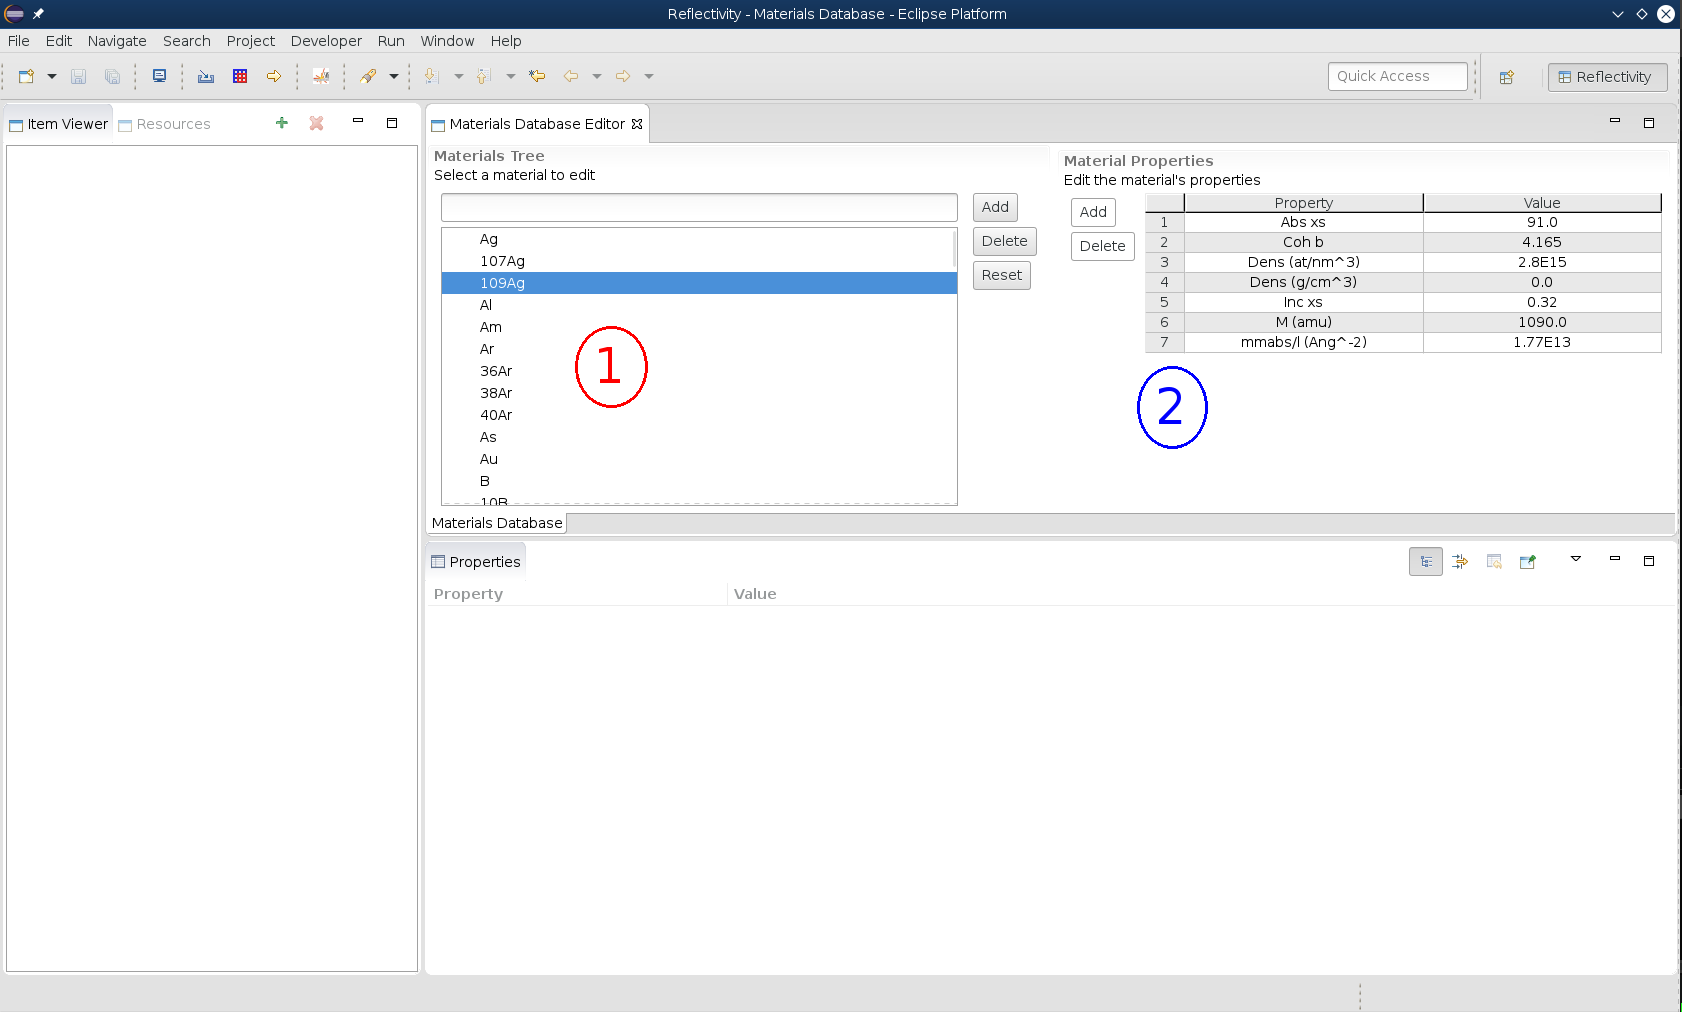
\includegraphics[width=10cm]{images/materialsDatabase_coated.png}
\caption{The materials database editor showing at 1 the list of materials in
the database and at 2 the properties for the selected material.}
\label{matDB}
\end{figure}

\section{Viewing the Data Outside the Simulator}
\label{viz}

The Reflectivity Simulator shows a lot of information in a tight space. It is
possible to view the final graphs for your data without the properties view,
Item Viewer, or Materials Table taking up valuable screen space. To do this,
choose Window$\rightarrow$Perspective$\rightarrow$Open
Perspective$\rightarrow$Other. A dialog will appear with a list of
\textit{Perspectives} that allow you to access the workbench in different ways.
Choose ``Resource (default)'' from the list.

The workbench will change when it loads the new perspective. On the left you
should see a ``Project Explorer'' menu with a folder in it called ``itemDB.''
You may also see views such as ``Outline'' or ``Tasks,'' both of which can be
safely minmized or closed. In the Project Explorer, open the itemDB folder and
double click one of the files that ends in *.csv. This will open a plot in the
middle of the screen, (fig. \ref{fullPlotView}).

\begin{figure}[!h]
\centering
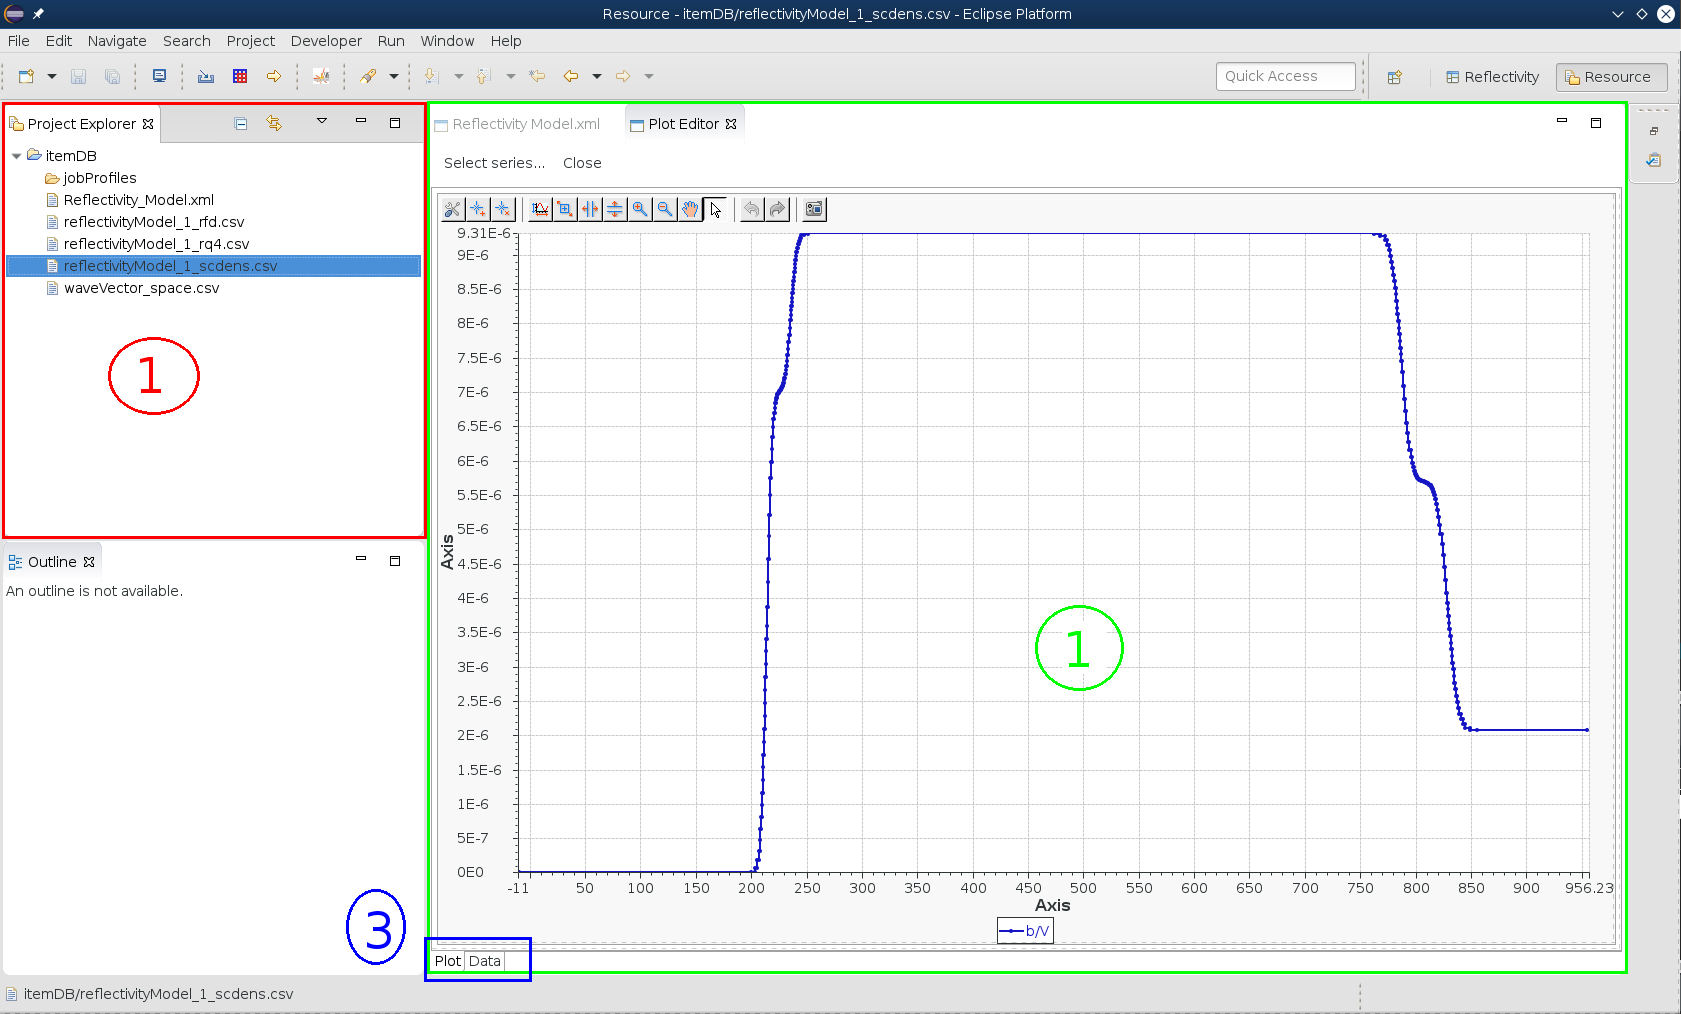
\includegraphics[width=10cm]{images/fullPlotView_coated.png}
\caption{The ``full plot view'' showing only the plot and no additional tables.
The red section labeled 1 shows the project explore and the CSV files in the
itemDB directory. The green section labeled 2 shows the scattering density for
the simulated material. The blue section labeled 3 shows two tabs that will let
you switch between the plot and the raw data.}
\label{fullPlotView}
\end{figure}

After you are finished you can switch back to the ``Reflectivity'' perspective
using the Window$\rightarrow$Perspective$\rightarrow$Open
Perspective$\rightarrow$Other menu or by clicking ``Reflectivity'' in the upper
right corner of the screen, if it is listed there.

\section{Exporting the Data}
\label{export}

The Resource Perspective discussed in section \ref{viz} can also be used to
export your data. You can do that either by using the ``data'' tab in the plot
through cutting and pasting, or by right-clicking on your file and choosing
Export. Alternatively, you can use your system's file browser to navigate to the
workspace directory that you specified in section \ref{gettingStarted}, where
you will find your data files in the itemDB subdirectory.
